\documentclass[11pt]{article}

\usepackage[margin=1in]{geometry}
\usepackage[T1]{fontenc}
\usepackage[utf8]{inputenc}
\usepackage{lmodern}
\usepackage{graphicx}
\usepackage{amsmath,amssymb,amsfonts}
\usepackage{algorithmic}
\usepackage{textcomp}
\usepackage{xcolor}
\usepackage[hidelinks]{hyperref}
\usepackage{booktabs}
\usepackage{multirow}
\usepackage[numbers]{natbib}
\usepackage{tikz}
\usetikzlibrary{positioning, arrows.meta, fit, matrix}

\hyphenation{poly-chron-isa-tion combi-nato-rial}

\begin{document}

\title{\Large\textbf{Permutations Are All You Need:\\Lookup-Table Transformers with Ranking Embeddings}}

\author{Eugene Izhikevich \and Anatoly Starostin}
\date{}

\maketitle

% ======================================================================
\begin{abstract}
Modern transformers represent tokens as real-valued vectors and manipulate them through matrix multiplications.
The \emph{Spiking Manifesto}~\cite{ref:manifesto} argues that the brain's computational advantage comes from the \emph{combinatorial} structure of spike orderings rather than from magnitudes, and proposes differentiable lookup tables (LUTs) indexed by pairwise comparisons as the corresponding computational primitive.
In this work we take that premise literally.
We build a transformer in which every learned operation depends only on the \emph{relative ordering} of its inputs --- not on any magnitudes --- and replace every matrix multiplication with a LUT.
The reformulation forces three substitutions: summation becomes concatenation, cosine similarity becomes Kendall-$\tau$ correlation, and matrix multiplication becomes an aggregation of lookup-table reads indexed by pairwise sign comparisons of the input.
Residual connections, which sum across layers, are replaced by layer-output concatenation into the vocabulary projection.
On a byte-level FineWeb benchmark at context length 128, our first purely combinatorial transformer reaches validation cross-entropy $1.239$ at 206M parameters, against a standard vanilla baseline at $1.203$ with 4.87M parameters.
We then introduce \emph{PermutationLUT}, a reparameterisation in which each LUT weight is a vote for a pairwise dominance relation rather than a real-valued output component.
Votes are sparse and tolerate aggressive quantisation.
Trained with 1-bit weights (\emph{BitPermutationLUT}) and a custom straight-through Adam variant, the model reaches $1.203$ --- matching the vanilla baseline --- at 205M bit-parameters ($\approx 25.6$\,MB bit-packed) plus a small number of full-precision scalars.
A multi-bit intermediate regime (\emph{MultiBitPermutationLUT}, e.g.\ 4-bit weights) is under study, motivated by the low precision of biological synapses.
Together these results show that a transformer can be made purely combinatorial --- and, once purely combinatorial, it compresses to single-bit weights at no loss of quality.
\end{abstract}

\medskip
\noindent\textbf{Keywords:} lookup tables, permutation embeddings, ranking attention, dominance projections, bit-quantisation, spiking neural networks, transformers


% ======================================================================
\section{Introduction}
\label{sec:intro}

The standard transformer~\cite{ref:vaswani} represents each token as a real-valued vector $\mathbf{x} \in \mathbb{R}^d$ and transforms sequences by linear projections and dot-product attention.
The information carried by an embedding lives in the \emph{magnitudes} of its components, and the basic computational unit is the multiply-accumulate operation.
This paradigm has scaled extraordinarily well, but it is tightly coupled to multiplication as a primitive, and it is not obviously the only way to build an expressive sequence model.

The \emph{Spiking Manifesto}~\cite{ref:manifesto} proposes a radically different view.
In biological spiking networks, information is carried by the \emph{relative timing} of spikes --- the combinatorial order in which neurons fire --- rather than by firing rates or voltage magnitudes.
Orderings offer factorial capacity: a sequence of $n$ distinguishable spikes admits $n!$ distinct patterns.
The underlying computation, the manifesto argues, can be realised through lookup tables indexed by pairwise timing comparisons, requiring only comparators and table reads instead of multiply-accumulate units.

This paper asks a single concrete question: \emph{can that combinatorial picture be carried through end-to-end into a working language model?}

The answer, we find, is yes, but it requires commitment.
A model that is ``mostly'' ordering-based --- that uses LUTs for projections but still sums real-valued activations, still uses cosine similarity inside attention, still adds residual streams --- is not actually combinatorial.
Magnitudes leak back in through the sums, and the model's capacity is again bounded by floating-point precision rather than by combinatorial structure.
Once one accepts the combinatorial premise literally, every arithmetic operation in the forward pass must be re-examined and, where necessary, replaced by a combinatorial analogue.

The paper follows that reformulation.
We start by reproducing the manifesto's LUT transformer and observing where magnitudes re-enter (Sections~\ref{sec:repro}--\ref{sec:leakage}).
We then lay out a small combinatorial vocabulary that replaces each offending arithmetic primitive (Sections~\ref{sec:framework}--\ref{sec:representations}).
We assemble a first purely combinatorial transformer from these pieces (Section~\ref{sec:first_combinatorial}), still large but competitive with a standard baseline.
We then introduce \emph{PermutationLUT}, a LUT variant in which each weight is a vote for a pairwise order relation (Section~\ref{sec:permlut}).
Votes are sparse and quantise aggressively: trained with 1-bit weights, \emph{BitPermutationLUT} matches the full-precision vanilla transformer on our benchmark at $\approx\!25.6$\,MB of bit-packed weights (Section~\ref{sec:bitperm}).
We close with a multi-bit intermediate regime motivated by biological synaptic precision (Section~\ref{sec:multibit}) and a short discussion (Section~\ref{sec:discussion}).

All code, experiments, and training logs are available at\\ \url{https://github.com/anatoli-starostin/spiky}.


% ======================================================================
\section{Background: Orderings, LUTs, and the Manifesto}
\label{sec:background}

\subsection{Permutation embeddings vs.\ magnitude embeddings}

A \emph{permutation embedding} carries information in the relative ordering of its components.
Given $\mathbf{x} \in \mathbb{R}^d$, let $\sigma_\mathbf{x}$ be the permutation that sorts $x_{\sigma(1)} \le x_{\sigma(2)} \le \cdots \le x_{\sigma(d)}$.
Two permutation embeddings are similar when many coordinate pairs agree on which side is larger --- the Kendall-$\tau$ rank correlation:
\begin{equation}
    \tau(\mathbf{x}, \mathbf{y}) \;=\; \frac{1}{\binom{d}{2}} \sum_{i<j} \mathrm{sgn}(x_i - x_j)\,\mathrm{sgn}(y_i - y_j).
    \label{eq:kendall}
\end{equation}
The encoding capacity of permutation embeddings is $d!$ (the number of distinct orderings), which grows factorially.
For $d = 16$, this gives $16! \approx 2 \times 10^{13}$ distinguishable patterns encoded in roughly $\log_2(16!) \approx 44$ bits.
A magnitude-based vector in $\mathbb{R}^{16}$ with float32 precision can represent $2^{512}$ distinct states --- vastly more --- but this capacity depends entirely on the ability to distinguish fine numerical differences.
In practice, operations like normalisation, quantisation, and additive noise destroy magnitude information, collapsing many of those $2^{512}$ states into equivalence classes.
The permutation capacity, by contrast, is robust: it depends only on the relative ordering, which is invariant to scaling, shifting, and any monotonic transformation of individual dimensions.

As shown in~\cite{ref:manifesto}, the number of $\varepsilon$-distinguishable vectors in $\mathbb{R}^n$ (the ANN capacity) scales as $e^{c(\varepsilon) \cdot n}$ where $c(\varepsilon) \sim \varepsilon^2$, while the combinatorial capacity of ordering-based representations scales as $m^n$ where $m \sim 1/\varepsilon$.
Since $1/\varepsilon \gg e^{\varepsilon^2}$ for any practical precision, the ordering-based capacity dominates.

\subsection{Lookup tables as a computational primitive}
\label{sec:lut_primitive}

Following~\cite{ref:manifesto}, we replace matrix multiplications with lookup tables indexed by pairwise comparisons.
A single table $S$ with $n_c$ \emph{anchor pairs} operates as follows:
\begin{enumerate}
    \item \textbf{Compare.} For each anchor pair $(a_k, b_k)$, $k = 1, \ldots, n_c$, compute $c_k = \mathbf{1}[x_{a_k} > x_{b_k}]$.
    \item \textbf{Index.} Form $j = \sum_{k=1}^{n_c} c_k \, 2^{k-1} \in \{0, \ldots, 2^{n_c} - 1\}$.
    \item \textbf{Lookup.} Retrieve the weight vector $S_j \in \mathbb{R}^{n_\mathrm{out}}$.
\end{enumerate}
The output of a multi-table module with $T$ tables is the sum
\begin{equation}
    \mathbf{y} = \sum_{t=1}^{T} S_{t,\,H_t(\mathbf{x})}
    \label{eq:lut}
\end{equation}
where $H_t(\mathbf{x})$ is the compare-and-index hash function for table $t$.
We refer to $n_c$ as \textbf{nap} (number of anchor pairs) and $T$ as \textbf{tph} (tables per head).
Since~\eqref{eq:lut} is piecewise constant, we train it with surrogate gradients~\cite{ref:manifesto}: each comparison receives an ``uncertainty'' $U(\delta_k) = \tfrac{1}{2(1+|\delta_k|)}$ that is large near the decision boundary, and the gradient carrier is the difference between the selected table entry and the nearest alternative (obtained by flipping the least-confident bit).


% ======================================================================
\section{Experimental setup}
\label{sec:setup}

\paragraph{Data.}
We use a 234\,MB subset of FineWeb~\cite{ref:fineweb}, byte-level tokenised with vocabulary $V = 257$ (256 byte values plus a beginning-of-sequence token).

\paragraph{Benchmark.}
All reported results use a common fixed protocol: context length $T = 128$ tokens, 100\,000 training steps, batch size $32$, Adam~\cite{ref:adam} at peak learning rate $10^{-3}$ with cosine schedule (10\% linear warmup, decaying to 10\% of peak).
Training and evaluation run on a single NVIDIA H100 80\,GB.
Validation loss is mean per-token cross-entropy on 10\,000 held-out test regions, evaluated every 1\,000 steps; we report the best validation value.
The fixed protocol removes scale and recipe as a confounder across architecture comparisons.

\paragraph{Vanilla baseline.}
Our reference is a standard causal transformer with $d_{\mathrm{model}} = 256$, 4 attention heads, 6 layers, feed-forward expansion factor 4, and fused QKV --- 4.87M parameters in float32.
Under the protocol above it reaches validation cross-entropy \textbf{1.203}.
Every combinatorial model in this paper is compared against this single number.


% ======================================================================
\section{Reproducing the manifesto model}
\label{sec:repro}

Our first step was to reproduce the manifesto's proposed architecture --- or, more precisely, a variant of it shared directly by one of the authors of~\cite{ref:manifesto}.
To run experiments at scale we built \texttt{spiky}, a small PyTorch library with fused CUDA kernels for the pair-comparison indexing and the multi-table accumulation of~\eqref{eq:lut}.
The reproduction is a six-layer transformer in which attention scores, value projections, and the feed-forward blocks are all realised as multi-head LUT modules; residual connections are retained.

Qualitatively, the result confirms the manifesto's claim: a model built from pairwise comparators and table reads can match a strong vanilla transformer on a language-modelling task.
Quantitatively, the reproduction is dramatically less parameter-efficient.
Reaching competitive loss required more than an order of magnitude more parameters than the vanilla baseline.
The rest of this paper is concerned with explaining that gap and closing it --- and, as it turns out, with a stronger claim about what kind of weights the combinatorial primitives actually need.


% ======================================================================
\section{Magnitude leakage: why the reproduction is not purely combinatorial}
\label{sec:leakage}

Shrinking the reproduction model led, unexpectedly, to a \emph{theoretical} observation rather than an engineering one.
The manifesto's architecture is not, in fact, purely combinatorial.
Several operations in the forward pass still depend on magnitudes, and each of them re-introduces the dependence on floating-point precision that the combinatorial picture was meant to remove.

Three leakages are most visible.

First, the sum in~\eqref{eq:lut} is a real-valued sum.
Each table produces a vector in $\mathbb{R}^{n_\mathrm{out}}$, and the module output is the arithmetic sum of $T$ such vectors.
The sum of two orderings is not itself an ordering; it depends on the \emph{magnitudes} of the two summands.
If we treat the output of~\eqref{eq:lut} as a ranking --- and downstream LUTs do, because they apply further comparisons to it --- then the model's ordering structure is entangled with the scale of each table's contribution.

Second, attention in the original manifesto-style architecture is a standard dot-product: scores are $\mathbf{q}^\top \mathbf{k}$, softmaxed, and used to weight values.
The dot product is a magnitude operation.
Kendall-$\tau$, the natural ordering-based similarity~\eqref{eq:kendall}, is \emph{not} the dot product of raw embeddings.

Third, residual connections sum a LUT output with the previous layer's embedding.
Again this is a magnitude-dependent operation; the resulting vector's ordering depends on the relative scales of its addends.

Each of these leakages by itself is small, but together they mean the model's quality is constrained by the floating-point resolution of intermediate activations, not by the combinatorial structure of orderings.
In the remainder of the paper we take the combinatorial premise seriously and replace each of these operations with a combinatorial analogue.


% ======================================================================
\section{A combinatorial math framework}
\label{sec:framework}

If every learned operation must depend only on orderings, every arithmetic primitive in the forward pass needs a combinatorial substitute.
Three substitutions are enough to get a complete architecture.

\paragraph{Summation $\to$ concatenation.}
Summing two orderings is ill-defined: the resulting vector's order depends on magnitudes.
The combinatorial analogue is \emph{concatenation}: two $d$-dimensional orderings become a single $2d$-dimensional ordering that carries both, with the relative positions of the two halves determined by the construction rather than by an arbitrary sum of magnitudes.
This applies wherever the original architecture summed intermediate representations: across tables inside a LUT, across blocks for residual connections, and so on.
For small embedding dimensions ($d = 32$ in our experiments) concatenation is cheap.

\paragraph{Cosine $\to$ Kendall-$\tau$.}
The dot product of two real vectors is a magnitude similarity.
The ordering similarity is Kendall's $\tau$ \eqref{eq:kendall}.
Crucially, $\tau(\mathbf{x}, \mathbf{y})$ equals the cosine of two \emph{rank signatures} --- $\pm 1$ vectors indexed by dimension pairs --- so Kendall-$\tau$ attention can be computed by applying standard scaled dot-product attention (SDPA) to those signatures.
This is the trick that makes combinatorial attention practical on GPU tensor cores.

\paragraph{Matrix multiplication $\to$ aggregated LUT reads.}
A dense linear projection $\mathbf{y} = W\mathbf{x}$ is a magnitude operation.
Its combinatorial analogue is a multi-table LUT module of the form~\eqref{eq:lut}: each output coordinate is the aggregate of table entries retrieved by pairwise-comparison indices.
The module depends on $\mathbf{x}$ only through the signs of $n_c$ differences $x_{a_k} - x_{b_k}$; scaling $\mathbf{x}$ by any positive constant leaves the output unchanged.

With these three substitutions, every learned operation in a standard transformer has a combinatorial counterpart.
What remains is to pick the \emph{representation} of orderings that is convenient at each point.


% ======================================================================
\section{Two representations of orderings}
\label{sec:representations}

We use two equivalent but computationally distinct representations of an ordering on $d$ elements.

\paragraph{Materialised ranking.}
A float vector $\mathbf{x} \in \mathbb{R}^d$ is interpreted as an ordering: only the sort order $\sigma_\mathbf{x}$ matters, and the magnitudes exist to encode that order.
This is the same tensor shape as in a standard transformer; the only change is interpretive.

\paragraph{Dominance matrix.}
For the same ordering, the \emph{dominance matrix} has entries $D_{ij}(\mathbf{x}) = \mathrm{sgn}(x_i - x_j) \in \{-1, +1\}$; equivalently, its upper-triangular part gives a $\binom{d}{2}$-dimensional vector.
For $d = 32$ this is a 496-dimensional sparse pattern.
Dominance is redundant (any $d - 1$ non-conflicting entries determine the rest) but convenient: comparisons that would otherwise be separate operations are materialised as tensor coordinates.

\begin{figure}[!t]
\centering
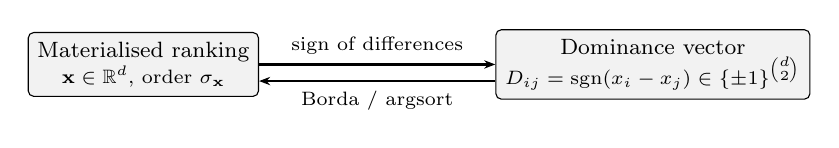
\begin{tikzpicture}[
    node distance=0.5cm,
    every node/.style={font=\footnotesize},
    block/.style={rectangle, draw, rounded corners=2pt, minimum width=2.5cm, minimum height=0.55cm, align=center, fill=#1},
    block/.default=blue!8,
    op/.style={block=green!8},
    arr/.style={-{Stealth[length=4pt]}, thick},
]
    \node[block=gray!10] (rank) {Materialised ranking\\ {\scriptsize $\mathbf{x} \in \mathbb{R}^d$, order $\sigma_{\mathbf{x}}$}};
    \node[block=gray!10, right=3.0cm of rank] (dom) {Dominance vector\\ {\scriptsize $D_{ij} = \mathrm{sgn}(x_i - x_j) \in \{\pm 1\}^{\binom{d}{2}}$}};
    \draw[arr] (rank.east) -- node[above, font=\scriptsize]{sign of differences} (dom.west);
    \draw[arr] ([yshift=-6pt]dom.west) -- node[below, font=\scriptsize]{Borda / argsort} ([yshift=-6pt]rank.east);
\end{tikzpicture}
\caption{The two representations of an ordering on $d$ elements that we use throughout the paper. A dense float vector encodes a ranking by its sort order. A dominance vector stores the pairwise sign matrix $\mathrm{sgn}(x_i - x_j)$. Conversion in one direction is the pairwise sign; conversion in the other is Borda counting (sum the dominance row) followed by LayerNorm. Both directions are used as layers inside the combinatorial transformer.}
\label{fig:representations}
\end{figure}

Conversion between the two is cheap.
Ranking $\to$ dominance is a pairwise sign; dominance $\to$ ranking is \emph{Borda counting} (sum each row of the dominance matrix) followed by a LayerNorm to stabilise scale.
Both directions are used as layers inside the combinatorial transformer (Figure~\ref{fig:representations}).

Why two representations?
Pairwise comparisons (including the LUT index function of Section~\ref{sec:lut_primitive}) are easier to express on dominance vectors.
Scaled dot-product attention, by~\eqref{eq:kendall}, is natural on dominance vectors: Kendall-$\tau$ is literally cosine similarity in that space.
On the other hand, the output of a LUT module is a materialised ranking: the aggregation of many table contributions naturally lives in $\mathbb{R}^{n_\mathrm{out}}$.
Each block of the combinatorial transformer therefore moves between the two representations at well-defined boundaries.


% ======================================================================
\section{First purely combinatorial transformer}
\label{sec:first_combinatorial}

We now have enough vocabulary to assemble a full transformer in which every learned operation depends only on orderings.

\subsection{Block structure}

Each of the $L = 6$ blocks has the same structure (Figure~\ref{fig:combinatorial_block}):
\begin{enumerate}
    \item \textbf{Q, K projections.} Apply a multi-head LUT (Section~\ref{sec:lut_primitive}) to $\mathbf{x}$, producing $H$ per-head queries and keys of dimension $d_{qk}$ as materialised rankings.
    \item \textbf{Dominance projection.} Convert Q and K to their dominance vectors in $\{-1, +1\}^{H \times \binom{d_{qk}}{2}}$.
    \item \textbf{Attention.} Standard causal SDPA on the dominance vectors. By~\eqref{eq:kendall} this is Kendall-$\tau$ attention.
    \item \textbf{V projection.} A multi-head LUT maps $\mathbf{x}$ to per-head value vectors; these are then converted to dominance.
    \item \textbf{Value aggregation.} Standard attention-weighted combination; the result is Borda-summed back to a materialised ranking and passed through LayerNorm.
    \item \textbf{Out-projection.} A multi-head LUT maps the $H \cdot d_v$-dimensional concatenation back to the block-output dimension $E$.
\end{enumerate}

\begin{figure}[!t]
\centering
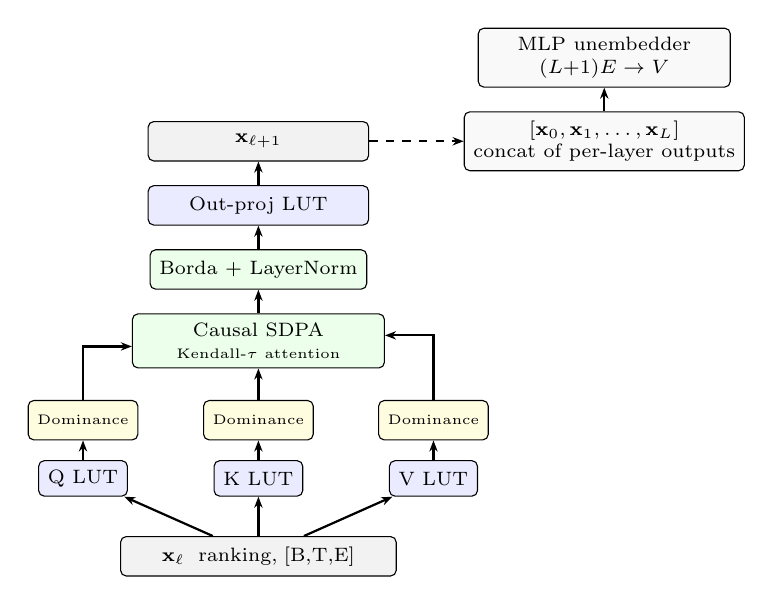
\begin{tikzpicture}[
    node distance=0.32cm,
    every node/.style={font=\scriptsize},
    block/.style={rectangle, draw, rounded corners=2pt, minimum width=2.8cm, minimum height=0.5cm, align=center, fill=#1},
    block/.default=blue!8,
    op/.style={block=green!8},
    dom/.style={block=yellow!12},
    smallblock/.style={rectangle, draw, rounded corners=2pt, minimum width=1.1cm, minimum height=0.45cm, align=center, fill=#1},
    smallblock/.default=blue!8,
    arr/.style={-{Stealth[length=4pt]}, thick},
]
    \node[block=gray!10, minimum width=3.5cm] (x) {$\mathbf{x}_\ell$ \;{\scriptsize ranking,\;[B,T,E]}};

    \node[smallblock, above left=0.5cm and -0.1cm of x] (q) {Q LUT};
    \node[smallblock, above=0.5cm of x] (k) {K LUT};
    \node[smallblock, above right=0.5cm and -0.1cm of x] (v) {V LUT};

    \node[dom, above=0.25cm of q, minimum width=1.1cm] (qd) {\tiny Dominance};
    \node[dom, above=0.25cm of k, minimum width=1.1cm] (kd) {\tiny Dominance};
    \node[dom, above=0.25cm of v, minimum width=1.1cm] (vd) {\tiny Dominance};

    \node[op, above=0.4cm of kd, minimum width=3.2cm] (sdpa) {Causal SDPA\\ \tiny Kendall-$\tau$ attention};

    \node[op, above=0.3cm of sdpa, minimum width=2.2cm] (borda) {Borda + LayerNorm};
    \node[block, above=0.3cm of borda] (op) {Out-proj LUT};
    \node[block=gray!10, above=0.3cm of op] (xout) {$\mathbf{x}_{\ell+1}$};

    \draw[arr] (x) -- (q);
    \draw[arr] (x) -- (k);
    \draw[arr] (x) -- (v);
    \draw[arr] (q) -- (qd);
    \draw[arr] (k) -- (kd);
    \draw[arr] (v) -- (vd);
    \draw[arr] (qd.north) |- ([yshift=-2pt]sdpa.west);
    \draw[arr] (kd) -- (sdpa);
    \draw[arr] (vd.north) |- ([yshift=2pt]sdpa.east);
    \draw[arr] (sdpa) -- (borda);
    \draw[arr] (borda) -- (op);
    \draw[arr] (op) -- (xout);

    % concat branch
    \node[block=gray!5, right=1.2cm of xout, minimum width=3.2cm, align=center] (cat)
        {$[\mathbf{x}_0, \mathbf{x}_1, \ldots, \mathbf{x}_L]$ \\ {\scriptsize concat of per-layer outputs}};
    \node[block=gray!5, above=0.3cm of cat, minimum width=3.2cm, align=center] (mlp)
        {MLP unembedder\\ {\scriptsize $(L{+}1)E \to V$}};
    \draw[arr, dashed] (xout.east) -- (cat.west);
    \draw[arr] (cat) -- (mlp);
\end{tikzpicture}
\caption{A single block of the first purely combinatorial transformer. Every learned module is a LUT; every attention step operates on dominance vectors (yellow), where cosine similarity equals Kendall-$\tau$. There is no residual connection: instead of summing each block's output back onto the stream, all per-layer outputs are concatenated at the top and projected to the vocabulary.}
\label{fig:combinatorial_block}
\end{figure}

\subsection{Concatenation in place of residuals}

There are no residual connections anywhere in the architecture.
The per-layer outputs $\mathbf{x}_0, \mathbf{x}_1, \ldots, \mathbf{x}_L$ are instead \emph{concatenated} at the top of the stack and passed through a two-layer MLP unembedder that emits vocabulary logits.
This is the ``summation $\to$ concatenation'' substitution of Section~\ref{sec:framework} applied to the inter-layer residual stream.
It is cheap because the per-layer embedding dimension is $E = 32$: concatenating $L + 1 = 7$ layers gives a 224-dimensional vector, small enough that the MLP unembedder remains a negligible fraction of the total parameter count.

\subsection{Result}

\begin{table}[!t]
\caption{First purely combinatorial transformer versus vanilla baseline, byte-level FineWeb at context length 128, 100\,000 steps.}
\label{tab:first_combinatorial}
\centering
\begin{tabular}{lrr}
\toprule
Model & Parameters & Val loss \\
\midrule
Vanilla transformer (float32)             & 4.87\,M    & \textbf{1.203} \\
First purely combinatorial (multi-head LUT, float32) & 205.6\,M   & \textbf{1.239} \\
\bottomrule
\end{tabular}
\end{table}

Under the protocol of Section~\ref{sec:setup}, the first purely combinatorial transformer reaches validation cross-entropy $1.239$ at $205.6$M parameters (Table~\ref{tab:first_combinatorial}), against the vanilla baseline of $1.203$ at $4.87$M.
The model is competitive --- the gap is $0.036$ nats per token --- but large: roughly $42\times$ more parameters than the baseline.
This is the weight-reduction problem that motivates the rest of the paper.


% ======================================================================
\section{PermutationLUT: voting in dominance space}
\label{sec:permlut}

The weight inflation of the first combinatorial model has a specific source.
A multi-head LUT writes its output directly as a materialised ranking: each of the $T \cdot 2^{n_c}$ table entries is a real-valued vector in $\mathbb{R}^{n_\mathrm{out}}$ whose magnitude matters, because downstream LUTs will read it through further comparisons.
Getting the \emph{order} of a sum of many such vectors to be consistent therefore requires each individual entry to be tuned with high precision.
The weights carry more information than the combinatorial semantics actually use.

\emph{PermutationLUT} is a reparameterisation designed to make the weight precision match the semantics.
Each weight in the table is reinterpreted as a \emph{vote} for a single pairwise dominance relation in the output space --- a statement that, for the given compare-and-index pattern, element $i$ of the output should rank above element $j$.
The LUT forward pass is:
\begin{enumerate}
    \item \textbf{Index.} Compute the compare-and-index hash $H_t(\mathbf{x})$ as in~\eqref{eq:lut}.
    \item \textbf{Rational activation.} Each selected weight $w$ is pushed through a soft-rational $v = \tfrac{1}{2} \cdot w / (T + |w|)$.
    \item \textbf{Scatter.} The activation is \texttt{scatter\_add}'ed into an accumulator indexed by the dominance coordinate $(i, j)$ that the weight votes for.
    \item \textbf{Borda + LayerNorm.} The resulting dominance accumulator is converted to a materialised ranking by Borda counting and LayerNorm.
\end{enumerate}
The number of pair coordinates available to vote on is $\binom{n_\mathrm{out}}{2}$; for $n_\mathrm{out} = 32$ this is 496.
This is larger than the ambient embedding dimension of a ranking, but votes are \emph{sparse}: most tables write into only a small subset of pair coordinates, so the effective degrees of freedom per weight are small and the aggregate signal-to-noise ratio is high.

The reparameterisation is sign-preserving and bounded: a weight's contribution to the output is a bounded monotonic function of its scalar value.
In contrast to the original multi-head LUT, a small perturbation of a weight produces a small, well-scaled perturbation of the output dominance vector.
This is what makes aggressive quantisation practical in the next section.

\begin{table}[!t]
\caption{PermutationLUT results, same protocol as Table~\ref{tab:first_combinatorial}.}
\label{tab:permlut}
\centering
\begin{tabular}{lrr}
\toprule
Model & Parameters & Val loss \\
\midrule
Vanilla transformer (float32)      & 4.87\,M   & \textbf{1.203} \\
First combinatorial (multi-head LUT)& 205.6\,M  & 1.239 \\
PermutationLUT (float32)            & 206.4\,M  & \textbf{1.226} \\
\bottomrule
\end{tabular}
\end{table}

Replacing every multi-head LUT in the combinatorial transformer with a PermutationLUT at matched parameter count gives validation loss $1.226$ (Table~\ref{tab:permlut}) --- a modest improvement over the materialised-ranking LUT.
The important property is not the small absolute gain but the fact that the reparameterisation made each weight an independent bounded scalar whose role is to nudge one pairwise dominance relation.
That is what lets us discard almost all of its precision.


% ======================================================================
\section{BitPermutationLUT: extreme quantisation}
\label{sec:bitperm}

Because each PermutationLUT weight is a vote rather than a real-valued output component, it tolerates aggressive quantisation.
\emph{BitPermutationLUT} takes the limit: each weight is stored as a single signed bit.

\subsection{Training with 1-bit weights}

Gradient descent needs continuous parameters, so we keep a low-precision latent weight $\tilde{w}$ per LUT entry during training (bfloat16 in our experiments) and pack its sign as the active 1-bit weight on every forward pass.
The forward evaluates the rational activation of Section~\ref{sec:permlut} at the \emph{packed} weight; the backward uses a straight-through estimator on the latent.
All matrix operations are fused CUDA kernels operating directly on the 1-bit packed representation.

A standard Adam optimiser cannot be used naively: Adam's second-moment estimate depends on the continuous latent, but the effective parameter is a step function of it, so most latent updates do not change the active weight at all.
We introduce a custom \emph{BitPermutationLUT optimiser}, a minimal Adam variant that (i) maintains first- and second-moment statistics on the continuous latent, (ii) applies the standard Adam update rule to the latent, and (iii) re-packs the sign after every step.
A straight-through gate suppresses moment updates when the latent is saturated far from the decision boundary, preventing drift in the Adam denominators.
At the end of training the latent is discarded; only the 1-bit packed weight is kept for inference.

\subsection{Result: matching vanilla with single-bit weights}

\begin{table}[!t]
\caption{Main result. BitPermutationLUT matches the vanilla baseline at $\approx 25.6$\,MB of bit-packed weights plus a small set of full-precision scalars (attention scale, LayerNorm affines, and the unembedder). Same protocol as Table~\ref{tab:first_combinatorial}. Storage columns quote packed weight bytes only; all four models run at the same context and step budget.}
\label{tab:bitperm}
\centering
\begin{tabular}{lrrr}
\toprule
Model & Bit-params & FP params & Val loss \\
\midrule
Vanilla transformer (float32)          & --          & 4.87\,M    & \textbf{1.203} \\
First combinatorial (multi-head LUT)    & --          & 205.6\,M   & 1.239 \\
PermutationLUT (float32)                & --          & 206.4\,M   & 1.226 \\
\textbf{BitPermutationLUT (1-bit)}      & \textbf{$\approx 205$\,M}   & \textbf{0.38\,M}    & \textbf{1.203} \\
\bottomrule
\end{tabular}
\end{table}

The main result of the paper is in the last row of Table~\ref{tab:bitperm}.
At equivalent capacity to the PermutationLUT transformer, the BitPermutationLUT model reaches validation cross-entropy $1.203$ --- equal to the vanilla baseline to three decimal places --- with approximately $205$\,M bit-packed weights ($\approx 25.6$\,MB) and $0.38$\,M full-precision scalars covering only the attention scale, LayerNorm affines, and the unembedder.
There is no measurable quality loss from restricting the LUT weights to one bit each.

Two observations are worth stating explicitly.
First, the vanilla baseline stores $4.87$\,M float32 weights ($\approx\!19.5$\,MB), so the bit-packed combinatorial transformer is \emph{comparable in raw weight storage} despite nominally having $42\times$ more ``weights.''
Second, and more importantly, the bit-packed model's forward pass requires only comparators, table reads, and signed additions --- no multiply-accumulate units --- for the bulk of its computation.
The small full-precision residue is confined to a handful of scalars (the learnable attention temperature and LayerNorm affines) and to the final MLP unembedder, which would admit the same treatment but is not on the critical path of this paper.


% ======================================================================
\section{MultiBitPermutationLUT: an intermediate regime}
\label{sec:multibit}

Going from full precision to one bit is the extreme of the quantisation spectrum.
There is a natural intermediate: \emph{MultiBitPermutationLUT}, where each weight is stored as a signed $K$-bit integer for small $K \in \{2, 4, 8\}$.
The mechanics are the same as in Section~\ref{sec:bitperm} --- bfloat16 latent, packed active weight, straight-through Adam --- but the pack kernel quantises to $2^K$ levels instead of two, using a midrise quantiser (no level at zero) together with a learned per-pair bias that compensates for the midrise shift.

Two motivations make this regime interesting.
The first is biological: real synapses are not binary but they are also not high precision; a small number of bits per synapse is the working assumption of most neuromorphic models.
The second is purely engineering: operations that are dominated by a wide fan-in (for example the out-projection in our architecture, which aggregates across four heads) benefit from a few extra bits of per-vote resolution even when the rest of the network is happy with one.

Full-scale results in this regime at the context length and training budget of Section~\ref{sec:setup} are still being collected.
Preliminary runs at reduced scale indicate that the midrise quantiser is important for bootstrapping (a level at zero creates a dead-zone in the early-training gradient) and that mixed-precision configurations, in which only the out-projection uses $K > 1$, are competitive with full-bit models at a small fraction of the storage.
We defer detailed numbers to future work.


% ======================================================================
\section{Discussion}
\label{sec:discussion}

\paragraph{The arc.}
Starting from the Spiking Manifesto, we reproduced its LUT transformer, observed that the reproduction was not in fact purely combinatorial, and used that observation to reformulate the architecture around three substitutions --- summation $\to$ concatenation, cosine $\to$ Kendall-$\tau$, matrix multiplication $\to$ LUT set --- applied uniformly throughout the forward pass.
The resulting first combinatorial transformer matched the vanilla baseline up to a $0.036$-nat gap, at the cost of $\sim\!40\times$ more parameters.
Reparameterising each LUT weight as a vote for a pairwise dominance relation (\emph{PermutationLUT}) made the weights independent bounded scalars, which then quantise cleanly to a single bit (\emph{BitPermutationLUT}) with no measurable quality loss.

\paragraph{What this says about representations.}
The fact that the final model closes the gap to vanilla \emph{only after} quantisation is worth interpreting carefully.
Nothing in the quantisation step adds capacity; it only removes precision.
The combinatorial reparameterisation is what makes the weights information-efficient, and the quantisation is a proof that the semantics of the model do not use the precision that the full-precision LUT parameters nominally carry.
In that sense the headline result is not really ``we match vanilla at 1 bit'' --- it is ``the combinatorial reformulation identifies the right representation, and once identified the precision requirement collapses.''

\paragraph{Hardware implications.}
A transformer whose forward pass is (comparators, table reads, LayerNorm, SDPA on $\pm 1$ vectors, and a small MLP) is a good fit for substrates that lack multiply-accumulate hardware or offer it only at high cost.
Neuromorphic and in-memory-compute platforms tend to have exactly that shape: cheap comparators and cheap table reads, scarce multiplies, scarce high-precision arithmetic.
We do not claim any specific hardware result in this paper; we claim only that the architectural side of that partnership has been built end-to-end and shown to be accuracy-neutral on a language-modelling benchmark.

\paragraph{Limitations.}
The benchmark is a 234\,MB subset of FineWeb at context length 128 and 100K steps; scaling to longer contexts and larger corpora is the obvious next step and not addressed here.
The full-precision residue (attention scale, LayerNorm affines, unembedder) is small but not zero, and folding it into the combinatorial primitives is future work.
The MultiBitPermutationLUT regime is reported only qualitatively at the protocol of Section~\ref{sec:setup}; full-scale numbers are in progress.


% ======================================================================
\section*{Acknowledgement}

The authors thank Vyacheslav Kluchnikov and Mikhail Burtsev for valuable discussions and feedback throughout this work.


% ======================================================================
\begin{thebibliography}{99}

\bibitem{ref:manifesto}
E.~Izhikevich, ``Spiking Manifesto,'' arXiv:2512.11843, Dec.~2025.

\bibitem{ref:vaswani}
A.~Vaswani, N.~Shazeer, N.~Parmar, J.~Uszkoreit, L.~Jones, A.~N.~Gomez, \L.~Kaiser, and I.~Polosukhin,
``Attention is all you need,'' in \emph{Proc.\ NeurIPS}, 2017.

\bibitem{ref:fineweb}
G.~Penedo, H.~Malartic, D.~Hesslow, R.~Cojocaru, A.~Cappelli, H.~Alobeidli, B.~Pannier, E.~Almazrouei, and J.~Launay,
``The FineWeb Datasets: Decanting the Web for the Finest Text Data at Scale,'' arXiv:2406.17557, 2024.

\bibitem{ref:adam}
D.~P.~Kingma and J.~Ba, ``Adam: A method for stochastic optimization,'' in \emph{Proc.\ ICLR}, 2015.

\bibitem{ref:polychrony}
E.~M.~Izhikevich, ``Polychronization: Computation with spikes,'' \emph{Neural Computation}, vol.~18, no.~2, pp.~245--282, 2006.

\bibitem{ref:lsh}
A.~Andoni and P.~Indyk, ``Near-optimal hashing algorithms for approximate near neighbor in high dimensions,'' in \emph{Proc.\ FOCS}, 2006.

\bibitem{ref:addernn}
H.~Chen, Y.~Wang, C.~Xu, B.~Shi, C.~Xu, Q.~Tian, and C.~Xu,
``AdderNet: Do we really need multiplications in deep learning?,'' in \emph{Proc.\ CVPR}, 2020.

\end{thebibliography}

\end{document}
